% --------------------------------------------------------------
% This is all preamble stuff that you don't have to worry about.
% Head down to where it says "Start here"
% --------------------------------------------------------------
 
\documentclass[12pt]{article}
 
\usepackage[margin=1in]{geometry} 
\usepackage{amsmath,amsthm,amssymb}
 \usepackage{graphicx}
\newcommand{\N}{\mathbb{N}}
\newcommand{\Z}{\mathbb{Z}}
 
\begin{document}
 
% --------------------------------------------------------------
%                         Start here
% --------------------------------------------------------------
 
\title{TSA 1 Report}
\author{Grant Yang \\ Period 1}
\maketitle

\section{Results}


\begin{figure}[h!]
    \centering
    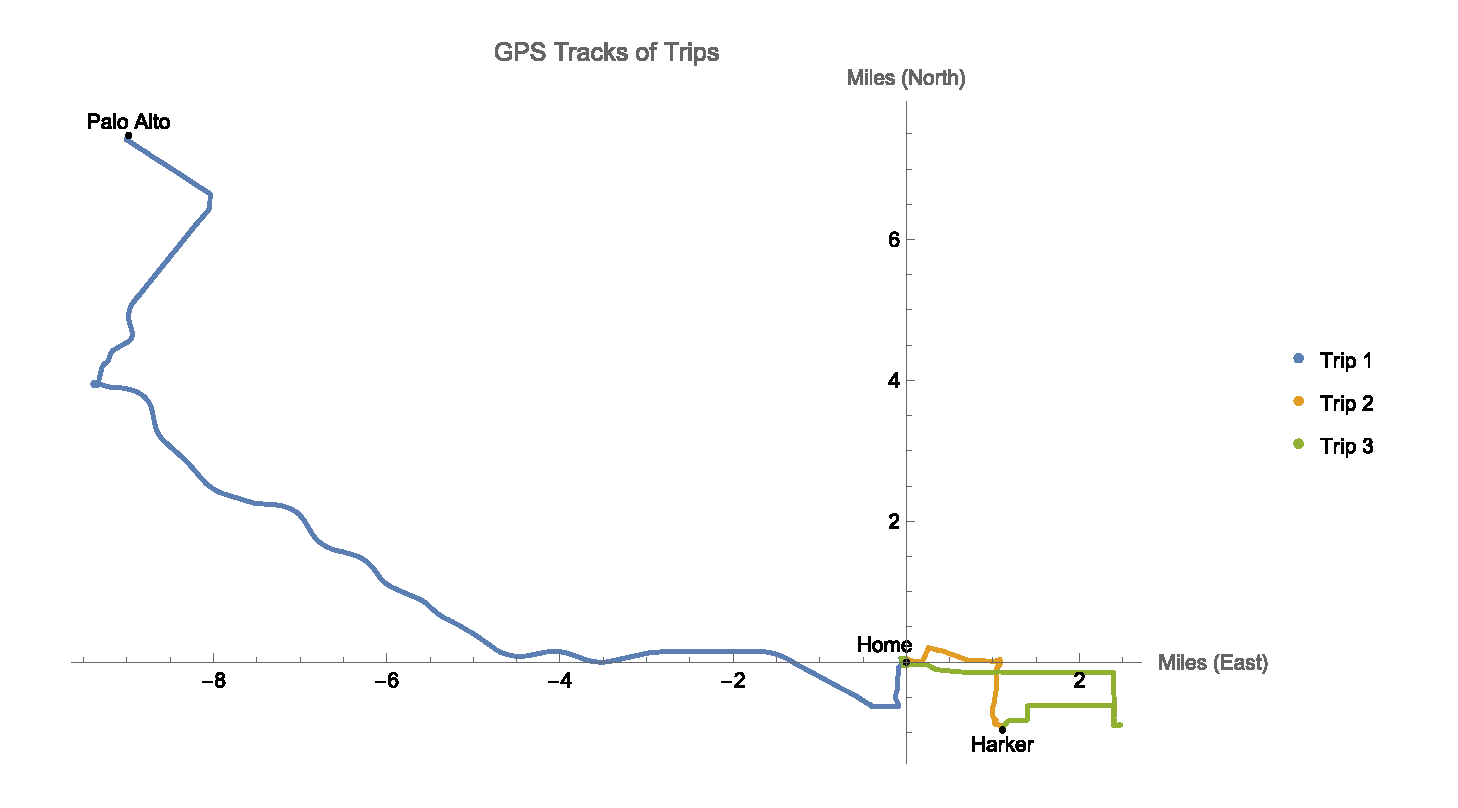
\includegraphics[width=1\linewidth]{tracks.pdf}
    \caption{GPS tracks of the three trips in the correct relative position and scale. Trip 1 went from Palo Alto to Home, trip 2 went from Home to Harker, and trip 3 went from Harker to Home.}
    \label{tracks}
\end{figure}
 
For three trips, we recorded GPS location data at a resolution of approximately one datapoint (a latitude and longitude pair) per second. Trip 1 was driven in an SUV from Palo Alto to my home, consisting of a section of driving on smaller suburban streets, followed by long stretch of moderate to heavy traffic on a freeway. Trip 2 was driven from my home to Harker in a sedan, avoiding all freeways and consisting of light traffic on smaller suburban roads. Trip 3 was driven from Harker to my home on the same day and in the same car, though we took a rather long detour to pick up food. Neither trip 2 nor trip 3 consisted of any driving on freeways.


\begin{table}[h!]
\centering
\begin{tabular}{|c|c|c|c|}
    \hline
     & Trip 1 & Trip 2 & Trip 3  \\
     \hline
     Datetime (PDT) & 2024.08.28 4 PM& 2024.09.03 at 7 AM& 2024.09.03 at 4 PM\\
     \hline
     Duration (min) & 34.7 & 7.8 & 24.5 \\
     \hline
     Distance (mi) &  16.9 & 2.4 & 5.6 \\
     \hline
     Displacement (mi) & 11.7 & $1.426^{*}$ & $1.467^{*}$ \\
     \hline
     Max Speed (mph) & 74.4 & 34.0 & 40.4 \\
     \hline
     Avg Speed (mph) & 29.0 & 18.3 & 13.6 \\
     \hline
     Speed stddev (mph) & 19.4 & 10.5 & 13.3 \\
     \hline
     
\end{tabular}

\caption{Calculated data values for the three trips. ($^{*}$) Theoretically, the values for the total displacements for trips 2 and 3 should agree, as they share the same endpoints. However, we observe an error equivalent to about $200\,\text{ft}$ between them, which is far more than our estimated GPS error of $30\,\text{ft}$ from our calibration. This discrepancy could be explained by the fact that we are numerically integrating displacements to calculate total displacement, and in that numerical integration, we are approximating the surface of the Earth as being completely flat within each time step. }
\label{table:2}
\end{table}

\newpage 
From these data, we can see that trip 3 had the greatest variation in speed relative to average speed, as a substantial amount of time was spent not moving while we were waiting for food. Because of the detour, trip 3 also has the greatest difference between total distance travelled and net displacement. Even when taking one of the most direct routes from home to school during trip 2, the layout of the roads forced us to drive nearly double the straight-line distance. During trip 1, which had the advantage of using a freeway, we still had to drive over 40\% more than the straight-line distance. Figure \ref{displ} below illustrates the time spent driving in the direction opposite to the ultimate destination across the three trips.

The greatest variation in speed overall happened during trip 1, the only trip where we drove on a highway. From the figure \ref{speeds} below, we see that while the speeds during trip 2 and 3 often drop to zero at stoplights, the speed during the highway section of trip 1 consistently remains above 20 mph from about 600 to 1300 seconds. From 1300 to about 1700 seconds, the traffic on the freeway grew more intense, and speed dropped to as low as 6 mph at some points, though it still always remained above zero.

While the instantaneous speed data are very noisy, we can integrate and obtain figure \ref{dists} to see the long term trends much more clearly. From this figure, we can see how the profiles of all three trips match very closely for the first 5 minutes, as they all initially started in the same types of suburban neighborhoods. Trip 3 clearly has the longest stretches of time spent at a standstill, and it quickly falls behind the other two trips and has a much lower average speed.


 \begin{figure}[h!]
     \centering
     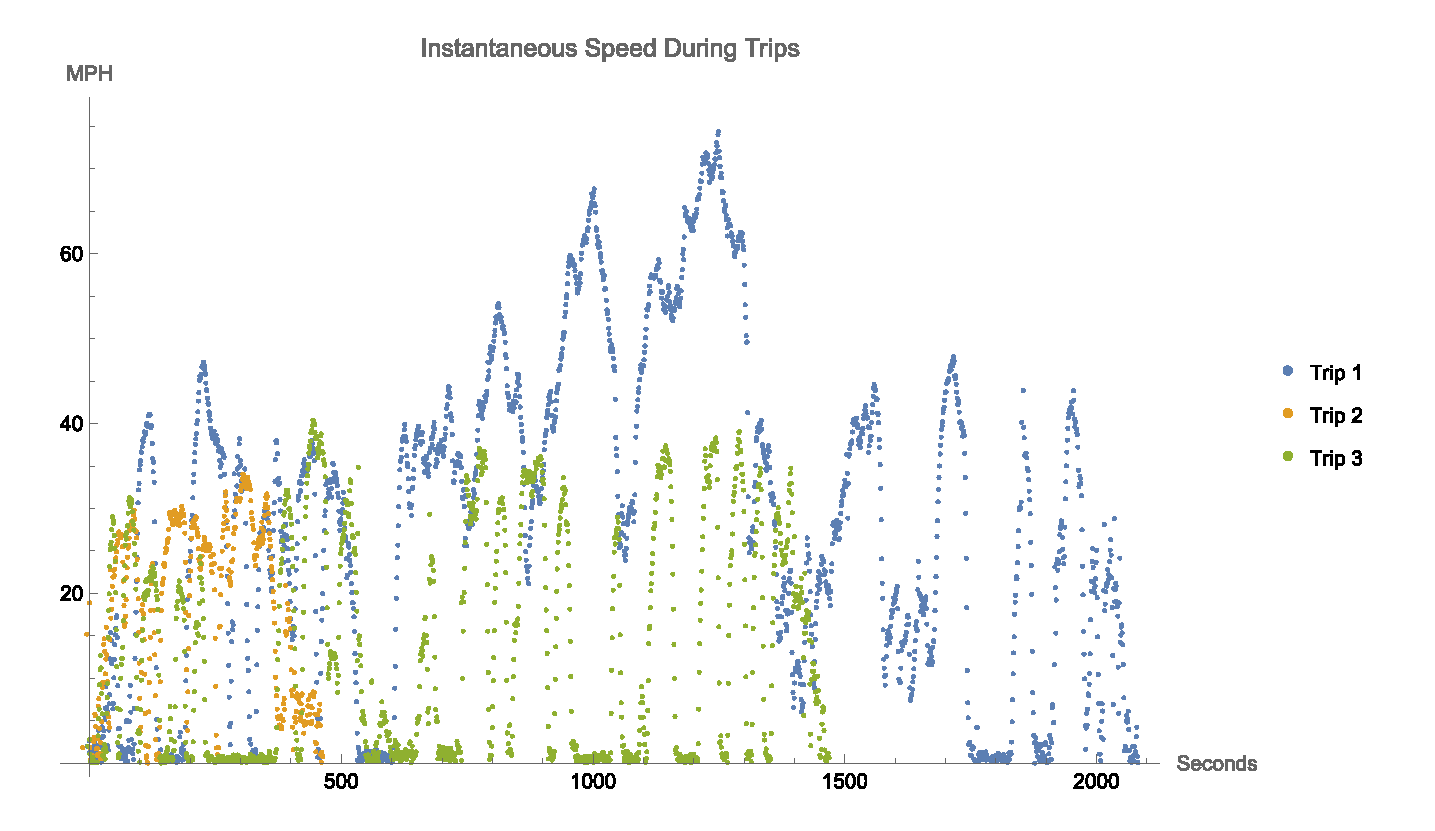
\includegraphics[width=0.9\linewidth]{speed.pdf}
     \caption{Instantaneous speed across all three trips. Note that the speed during Trip 1 consistently remains above 20 mph during the freeway section at around 1000 seconds, something not seen during the other trips.}
     \label{speeds}
 \end{figure}

  \begin{figure}[h!]
     \centering
     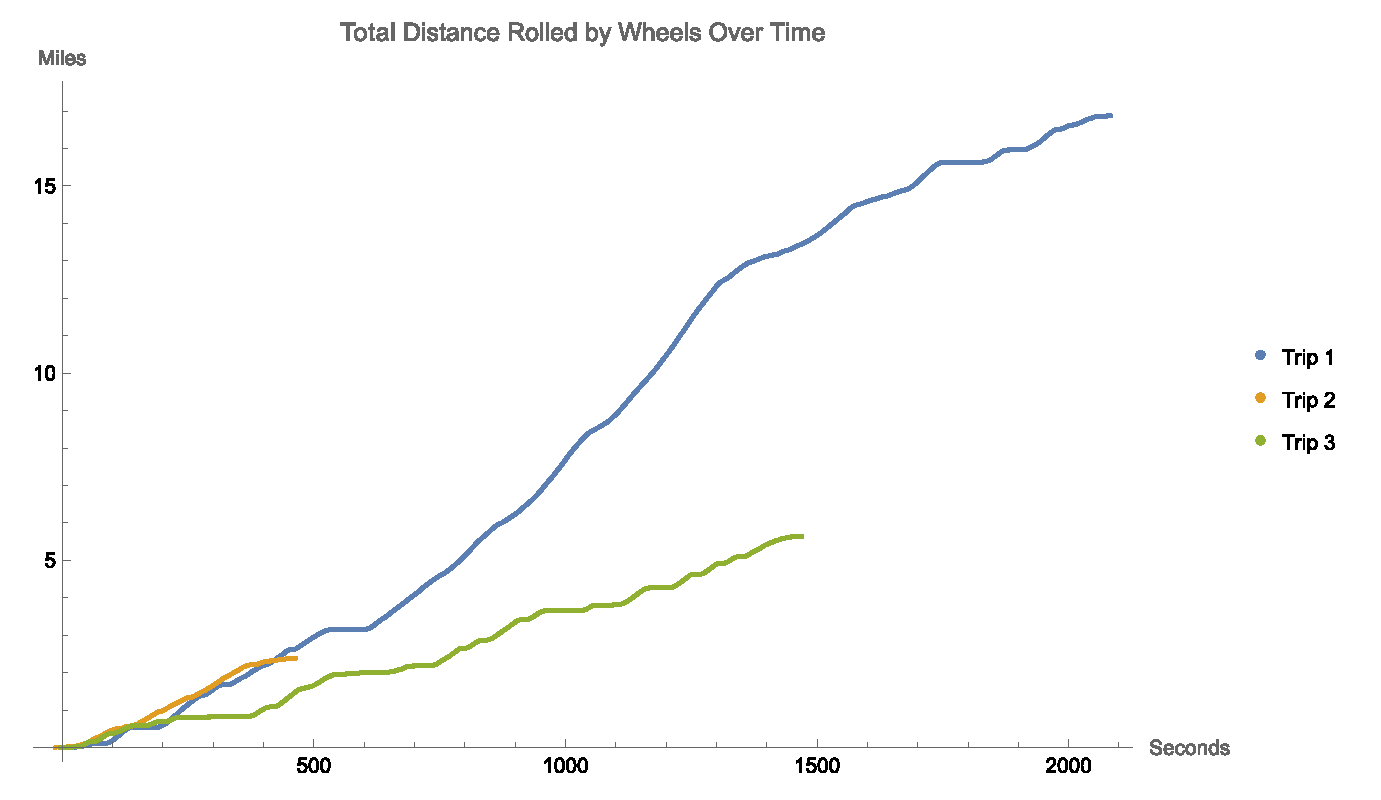
\includegraphics[width=0.9\linewidth]{dist.pdf}
     \caption{Total distance travelled over time. This figure is the time integral of figure \ref{speeds}. Note the similar profiles for the first 5 minutes of all trips, the steeper slope during the highway segment of trip 1, and the times spent stopped during all trips.}
     \label{dists}
 \end{figure}

   \begin{figure}[h!]
     \centering
     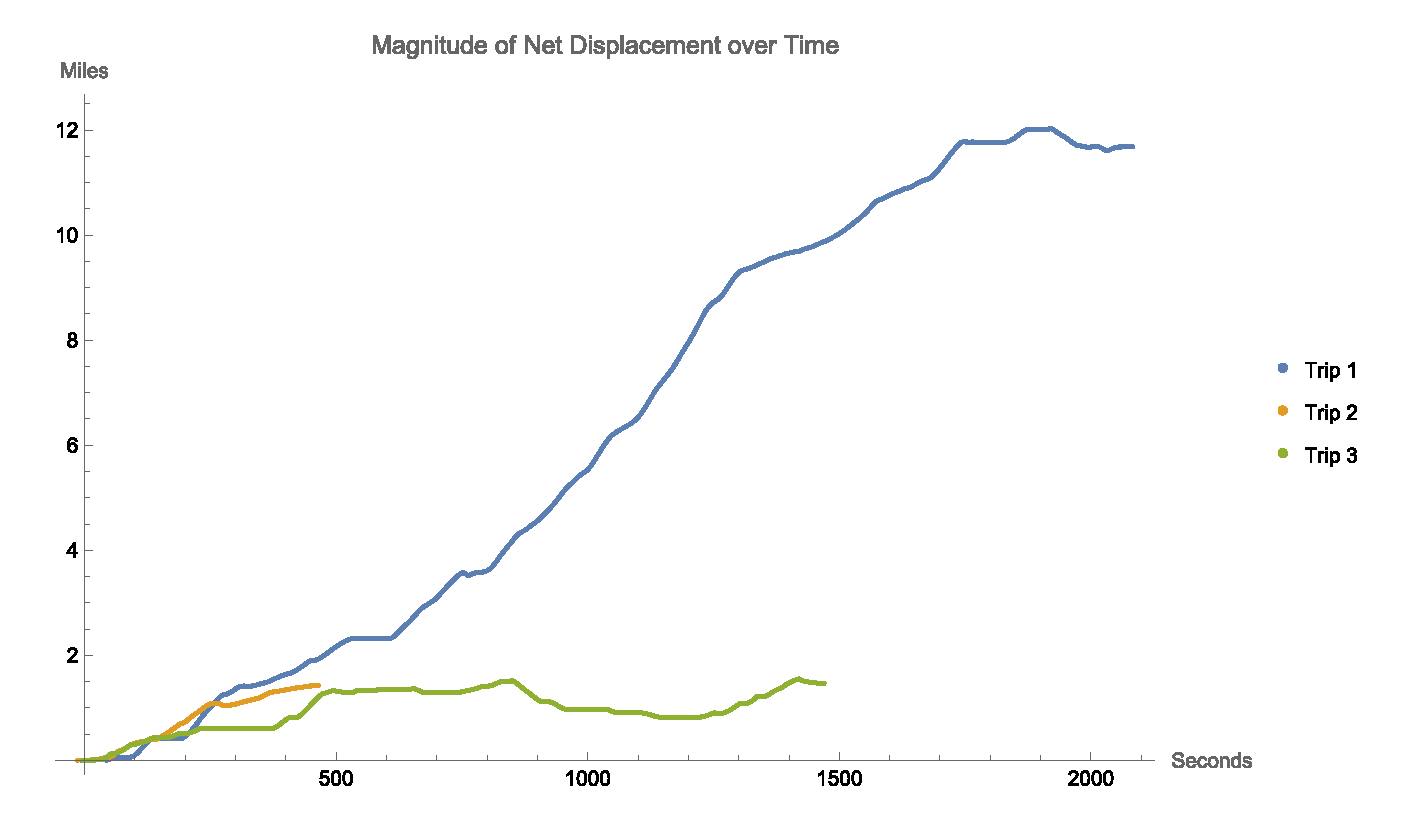
\includegraphics[width=0.9\linewidth]{displ.pdf}
     \caption{Magnitude of net displacement over time. Note the time spent driving in the direction opposite the final destination due to the inefficient layout of roads, especially after the detour on trip 3.}
     \label{displ}
 \end{figure}
\end{document}
